% MplTplt - Yet another LaTeX template for Modern Physics Lab, PKU.
% Copyright (C) 2014 Huang Kangjing and contributors

% This work is completely rewritten basing on the work of Cao Chuanwu
% and Sun Sibai, with texts in the template originally coming from the
% Modren Phys. Lab.

% This file is released under the MIT license.
%
% Permission is hereby granted, free of charge, to any person obtaining a copy
% of this software and associated documentation files (the "Software"), to deal
% in the Software without restriction, including without limitation the rights
% to use, copy, modify, merge, publish, distribute, sublicense, and/or sell
% copies of the Software, and to permit persons to whom the Software is
% furnished to do so, subject to the following conditions:
% 
% The above copyright notice and this permission notice shall be included in
% all copies or substantial portions of the Software.
% 
% THE SOFTWARE IS PROVIDED "AS IS", WITHOUT WARRANTY OF ANY KIND, EXPRESS OR
% IMPLIED, INCLUDING BUT NOT LIMITED TO THE WARRANTIES OF MERCHANTABILITY,
% FITNESS FOR A PARTICULAR PURPOSE AND NONINFRINGEMENT. IN NO EVENT SHALL THE
% AUTHORS OR COPYRIGHT HOLDERS BE LIABLE FOR ANY CLAIM, DAMAGES OR OTHER
% LIABILITY, WHETHER IN AN ACTION OF CONTRACT, TORT OR OTHERWISE, ARISING FROM,
% OUT OF OR IN CONNECTION WITH THE SOFTWARE OR THE USE OR OTHER DEALINGS IN
% THE SOFTWARE.
%

% This template depends on the "revtex4.1" package from APS Journals
% <http://publish.aps.org/revtex/revtex-faq>, and the Chinese handling
% is done with XeLaTeX engine and package "xeCJK". Please ensure these
% packages are available in your chosen Tex software distribution.

% Document created using this template should be compiled with XeLaTeX
% engines rather than plain LaTeX or plain TeX engines.

% The non-ASCII texts of this template is encoded in UTF-8 encoding.
% Please note that XeLaTeX only accepts UTF-8 encoded documents, so
% set your editor to use UTF-8 while creating documents with this template.

% Recommended TeX software distribution to use with this template is
% Tex Live developed by the TeX User Group (TUG), please visit the home
% page of the distribution <https://www.tug.org/texlive/> for further details.

% NOTE THAT IMPORTANT INSTRUCTIONS HAS BEEN WRITTEN AS UPPERCASE COMMENTS
% IN THE TEXT, PLEASE READ THEM CAREFULLY AND FOLLOW THEM TO MAKE THE
% TEMPLATE WORK!

% Any further contributions to the template is welcome, please send
% pull requests through github or send mail to maintainer.

% For any other questions, please do not hesitate to contact maintainer.

% Current maintainer:
% Huang Kangjing <huangkangjing@gmail.com>

% Contributors:
% Sun Sibai <niasw@pku.edu.cn>
% Cao Chuanwu <>
% Huang Kangjing <huangkangjing@gmail.com>


\documentclass[aps,pre,12pt,preprint,onecolumn,showpacs,showkeys]{revtex4-1}

% Setting up Chinese handling.
\usepackage{fontspec,xeCJK}

% Setting up fonts.
% PLEASE MODIFY ALL THESE FONT NAMES ACCORDING TO YOUR FONT
% INSTALLATION AND PERFERENCE.

% Setting up main fonts and mono fonts.
\setmainfont{Liberation Serif}
\setmonofont{Liberation Mono}
% SimSun is required font for the main body of the text.
\setCJKmainfont[AutoFakeBold=5,AutoFakeSlant]{SimSun}
\setCJKmonofont[AutoFakeBold=2,AutoFakeSlant]{SimHei}

% Setting up alternative font families.
% Note that these three fonts below are required fonts in document
% title, section headings and figure captions.
\newCJKfontfamily\heiti[AutoFakeBold=2,AutoFakeSlant]{SimHei}
\newCJKfontfamily\fangsong[AutoFakeBold=5,AutoFakeSlant]{FangSong}
\newCJKfontfamily\kaiti[AutoFakeBold=5,AutoFakeSlant]{KaiTi}

% Setting up paragraph indent.
\parindent 2em

% Setting up macros for Chinese-style font size setting.
\newcommand{\fseight}{\fontsize{5.02}{6.02}\selectfont}
\newcommand{\fsseven}{\fontsize{5.52}{6.62}\selectfont}
\newcommand{\fsssix}{\fontsize{6.52}{7.83}\selectfont}
\newcommand{\fssix}{\fontsize{7.53}{9.03}\selectfont}
\newcommand{\fssfive}{\fontsize{9.03}{10.84}\selectfont}
\newcommand{\fsfive}{\fontsize{10.54}{12.65}\selectfont}
\newcommand{\fssfour}{\fontsize{12.05}{14.45}\selectfont}
\newcommand{\fsfour}{\fontsize{14.05}{16.86}\selectfont}
\newcommand{\fssthree}{\fontsize{15.06}{18.07}\selectfont}
\newcommand{\fsthree}{\fontsize{16.06}{19.27}\selectfont}
\newcommand{\fsstwo}{\fontsize{18.07}{21.68}\selectfont}
\newcommand{\fstwo}{\fontsize{22.08}{26.50}\selectfont}
\newcommand{\fssone}{\fontsize{24.09}{28.91}\selectfont}
\newcommand{\fsone}{\fontsize{26.10}{31.32}\selectfont}
\newcommand{\fsszero}{\fontsize{36.14}{43.36}\selectfont}
\newcommand{\fszero}{\fontsize{42.16}{50.59}\selectfont}

% Replace words to Chinese corespondence.
\renewcommand\appendixname{附录}
\renewcommand\abstractname{}
\renewcommand\tablename{表}
\renewcommand\figurename{图}

% Replace words in revtex4-1 to Chinese corespondence.
\makeatletter
\def\@pacs@name{\heiti\fssfour \textbf{PACS码:}\normalfont}
\def\@keys@name{\heiti\fssfour \textbf{关键词:}\normalfont}
\def\Dated@name{日期:}
\def\Received@name{\fssfive 接收 }
\def\Revised@name{\fssfive 修订 }
\def\Accepted@name{\fssfive 采纳 }
\def\Published@name{\fssfive 发表 }
\makeatother

% Change label style of enumerate.
\renewcommand{\labelenumi}{\alph{enumi}.}

% Setting up geometry.
\usepackage{geometry}
\geometry{top=2.54cm,bottom=2.54cm,left=3cm,right=3cm}

% Setting up line space.
\usepackage{setspace}
\linespread{1.6}

% Setting up hyperreferences.
\usepackage{hyperref}
\hypersetup{colorlinks=true}

% Setting up styles for section headings.
\usepackage{titlesec}
\titleformat*{\section}{\bf\fangsong\fsfour}
\titleformat*{\subsection}{\bf\fangsong}

% Loading packages for image handling.
\usepackage{subfig}
\usepackage{graphicx,psfrag,epsfig}

% Setting up caption styles.
\usepackage{caption}
\DeclareCaptionFont{kaiti}{\kaiti}
\DeclareCaptionFont{bfheiti}{\bf\heiti}
\captionsetup{font=small,format=plain,labelfont=bfheiti,%
  textfont=kaiti,justification=raggedright,%
  singlelinecheck=false}

% Loading packages for math typings.
\usepackage{amsmath,amsfonts,amssymb,amsthm,bm,upgreek}
\usepackage[mathscr]{eucal}
\usepackage{siunitx}

\usepackage{listings}

\lstset{%
    breaklines=true,
    basicstyle=\fontspec{Liberation Mono}\footnotesize,
    commentstyle=\fontspec{Liberation Mono}\color{green},
    showspaces=false,
    stringstyle=\fontspec{Liberation Mono},
    numbers=left,
    numberstyle=\fontspec{Liberation Mono}\tiny,
    keywordstyle=\fontspec{Liberation Mono}\color{blue},
    title=\lstname,
    frame=L}

\begin{document}

% Title and author info.
\title{\bf\heiti\fsthree 磁光克尔效应\vspace{15mm}}
\author{\fangsong\fsfour 黄康靖\vspace{2mm}}
\affiliation{\normalfont\fssfour 2012级~~~~{masked student id}\vspace{2mm}}
\date{\today}
\keywords{磁光效应,克尔效应,磁滞回线,锁相放大器,微机控制,自动测量,微弱信号测量}
\email{huangkangjing@gmail.com}

% Abstract.
\begin{abstract}
  \vspace{10mm}
  \begin{spacing}{1.5}
    \fssfour
    1877年,克尔发现平面偏振光从光洁磁极表面反射时,偏振面会发生微小的偏转,后人称
    为克尔效应.克尔效应是磁光效应的一种,自发现以来,在物理学的各个分支学科与技术中,都
    有着广泛的应用.磁光克尔效应背后的机理值得研究.本实验通过光弹调制器调制从磁光
    克尔样品上,经极克尔效应反射回来的光线,并通过微机控制的锁相放大器测量微小信号
    ,测定了样品的克尔磁滞回线,并且计算得出了样品的饱和克尔转角与矫顽力.
  \end{spacing}
\end{abstract}

% The main body of the document goes from here.
\maketitle
\fssfour
\section{引言}

1845年,法拉第观察到平面偏振光在穿过在光的传播方向加有磁场的玻璃时,偏振面的角度
会发生旋转,是为法拉第效应.1877年,克尔发现平面偏振光从光洁磁极表面反射
时,偏振面会发生微小偏转,是为克尔效应.1896年,塞曼发现,当光源置于磁场中时,原来的一条谱
线会分裂成几条偏振化的谱线,是为塞曼效应.这些效应反映了物质磁化状态对其光学性质的
影响,被统称为磁光效应.

借助磁光效应可以用光学方法探测物质的磁化状态,亦可通过施加不同的外磁场来改变物质
对光场的响应行为来实现一些应用目的.因此,磁光效应在物理学的诸多分支和应用中都有着
重要的应用.

另一方面,由于磁光克尔效应观察的是样品表面的反射光,不要求样品透明,所以其适用范围
相对更宽.自上世纪50年代以来,磁光克尔效应及其相关技术在各个分支的物理学中,都得到
了充分的发展和应用.

本实验通过测量一个磁性薄膜的磁光克尔磁滞回线,研究了克尔效应的基本原理,探究了相关
的测量技术,并且测得了样品的饱和克尔转角值和矫顽力.

\section{原理}

\subsection{磁光效应的唯象理论}

光在介质分界面的反射与折射现象可以用菲涅尔公式准确地描述.而在光频段,相对磁导率可
以看作1,折射率由介电常数决定,因此,相关的推导可以从介电常数入手.

最一般的情况下,介电常数是一个复张量,可以记作
\begin{equation}
    \epsilon =
    \begin{pmatrix}
        \epsilon_{xx} &\epsilon_{xy} &\epsilon_{xz}\\ 
        \epsilon_{yx} &\epsilon_{yy} &\epsilon_{yz}\\ 
        \epsilon_{zx} &\epsilon_{zy} &\epsilon_{zz} 
    \end{pmatrix}
\end{equation}

假设在磁光介质中,只有磁化沿着$z$方向所引起的各向异性,那么由空间对称性分析和时间
反演不变性可以得到
\begin{equation}
    \epsilon = 
    \begin{pmatrix}
        \epsilon & \delta & 0 \\
        -\delta & \epsilon & 0 \\
        0 & 0 & \epsilon_z
    \end{pmatrix}
    = \epsilon_0 n^2
    \begin{pmatrix}
        1 & -iQ & 0 \\
        iQ & 1 & 0 \\
        0 & 0 & n_Z^2/n^2
    \end{pmatrix}
\end{equation}
其中$\epsilon_0$为真空介电常数,$n$为平均复折射率,是$\mathbf{M}$的偶函数,$Q =
\frac{-i\delta}{\epsilon_0n^2}$是$\mathbf{M}$的奇函数,称为复磁光系数.

采用新的坐标系,可以将介电常数张量对角化为:

\begin{equation}
    \epsilon = \epsilon_0n^2
    \begin{pmatrix}
        1 + Q & 0 & 0 \\
        0 & 1 - Q & 0 \\
        0 & 0 & n_z^2/n^2
    \end{pmatrix} = 
    \begin{pmatrix}
        n_+^2 & 0 & 0 \\
        0 & n_-^2 & 0 \\
        0 & 0 & n_z^2
    \end{pmatrix}
\end{equation}
其中$n_{\pm}^2 = n^2(1\pm Q)$

由于$Q\ll 1$,有
\begin{equation}
    n_{\pm} = n \sqrt{1\pm Q} \approx n(1 \pm \frac{Q}{2})
\end{equation}
\begin{equation}
    n = \frac{n_+ + n_-}{2}
\end{equation}

沿磁化强度方向传播的光的本征态为左旋或者右旋偏振光,对应的折射率之差为$nQ$.

考虑入射光垂直入射到介质表面时,产生的极克尔效应,按以上的推导以及菲涅尔公式,可以
得到,入射的线偏振光在经过克尔介质反射之后,将会成为长轴方向与原线偏振光有一定夹角
的椭圆偏振光,这一行为可以用复克尔转角表述:

\begin{equation}
    \widetilde{\theta_K}  = \theta_k + i \epsilon_k \approx - i \frac{nQ}{1 - n^2}
\end{equation}
其中,$\theta_k$为克尔转角,即为椭圆偏振光相对长轴转过的角度,而$\epsilon_k$则为克
尔椭偏率,为出射椭圆偏振光的椭偏率.

\subsection{磁光常数的动力学解释}

磁光常数的动力学解释可以由经典电动力学中的介质极化和色散的振子模型得到
\cite{Landau}\cite{mo},其表达式应为:
\begin{equation}
   Q = - \frac{2Ne^2\omega_0\omega_L/m\epsilon_0}{(\omega_0^2- \omega^2 -
       i\gamma\omega)\left[(\omega_0^2 - \omega^2 - i\gamma\omega) +
           \frac{Ne^2}{m\epsilon_0}\right]} 
\end{equation}

式中$\omega_0 = \sqrt{k / m}$为振子的固有频率,$\omega$为光场的振荡频率,而
$\omega_L = \frac{e}{2m}B$为电子轨道在外磁矩中的经典拉莫尔进动角频率.

\section{实验}

\subsection{实验装置}

实验装置的方框图如图~\ref{fig:inst}所示

\begin{figure}[htbp]
    \centering
    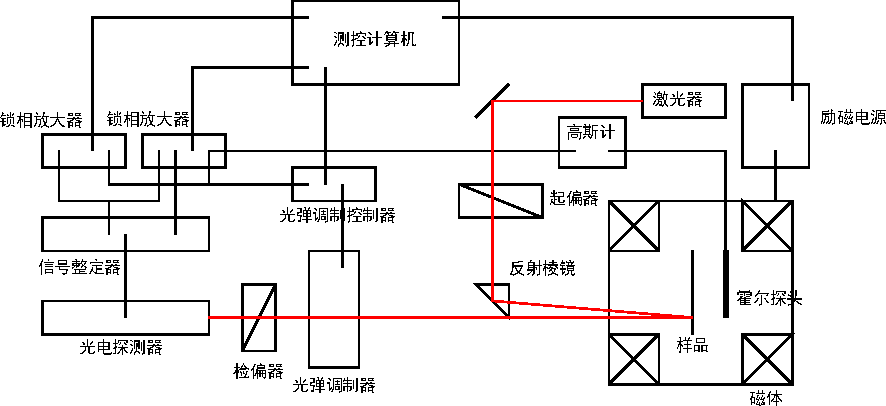
\includegraphics[width=\textwidth]{inst.pdf}
    \caption{\label{fig:inst}~此为实验装置的示意图,通过一台测控计算机,经COM口连
        接各测量设备,并利用锁相放大器的A/D转换功能,收集各模拟信号输出的探测器数
        据,再在计算机上通过程序控制,实现克尔磁滞回线的扫描测量.具体的测量原理参
        见\ref{sec:prin}}
\end{figure}

\subsection{实验具体原理与测量公式}

\label{sec:prin}

下面来简述一下上述实验装置的具体原理与测量公式.

在本实验的实验装置中,采用了锁相放大器作为光电探测器的放大设备,以及作为高斯计模拟
信号输出转换成计算机可以直接理解的数字信号输入这一转换桥梁的A/D转换器.为了能够实
现锁相放大器放大微小信号的功能,实验中测得的光强变化频率和锁定放大器的参
考信号频率之间必须具备确定的频率关系.实验通过光弹调制器的调制保证了这一点.

任何一个纯偏振态都可以表示为两个独立偏振模的叠加,如果以对应的独立偏振模为基,任何
纯偏振态都可以用一个二维矢量表示,而一个改变偏振态的线性光学器件的效应则可以用一
个二维矩阵表示,是为琼斯矩阵.

取光沿着$-z$方向传播,并且光弹调制器的振动轴沿着$x$方向,容易得出,光弹调制器与角度
为45度的检偏器的琼斯矩阵分别为.
\begin{equation}
    \begin{pmatrix}
        1 & 0 \\
        0 & e^{i\delta}
    \end{pmatrix} ,
    \begin{pmatrix}
        1/2 & 1/2 \\
        1/2 & 1/2
    \end{pmatrix}
\end{equation}
其中$\delta$为经过光弹调制器后,光的$y$方向电场分量相对于$x$方向电场分量的相位延
迟量.

当测量的是极克尔效应时,琼斯矩阵应该为
\begin{equation}
    \begin{pmatrix}
        r_F & -k \\
        k & r_F
    \end{pmatrix}
\end{equation}
将入射光的矢量乘上依次以上各个琼斯矩阵,并且
\begin{equation}
    \delta = \delta_0 \sin{\omega t}
\end{equation}
并对光强变化函数的结果作贝塞尔展开,可以得到:
\begin{equation}
    \begin{split}
        I(t) \approx  & \frac{r_F^2 + k^2}{2}(1 + 2\theta_k\cos{\delta} -
        2\epsilon_k\sin{\delta}) \\
         = & \frac{r_F^2 + k^2}{2}(1 + 2\theta_kJ_0(\delta_0) -
         4\epsilon_kJ_1(\delta_0)\sin{\omega t} +
         4\theta_kJ_2(\delta_0)\cos{2\omega t} + \dots)
    \end{split}
\end{equation}
如果取$\delta_0 = \num{2.405}$为零阶贝塞尔函数的零点,并测出光强信号的直流分量
$V_0$,一次谐波分量$V_{\omega}$,二次谐波分量$V_{2\omega}$,即有
\begin{equation}
    \theta_k = \frac{\sqrt{2}V_{2\omega}}{4V_0J_2(\delta_0)}
\end{equation}
\begin{equation}
    \epsilon_k = \frac{\sqrt{2}V_{\omega}}{4V_0J_1(\delta_0)}
\end{equation}

\subsection{实验测量}

在具体实验中,将会通过线性定标的方法,来标定克尔转角的测量,从而可以直接乘以系数得
到克尔转角的数值.

实验采用了\SI{632.8}{nm}的激光作为光源,测量了给定样品的克尔磁滞回线.

测量从\SI{-1000}{mT}开始,扫描到正向\SI{1000}{mT}后又回到\SI{-1000}{mT},每隔
\SI{50}{mT}测量一个点.

\section{实验结果及分析讨论}

实验通过程序自动测量得到的磁滞回线数据,绘制了线性插值的磁滞回线图线(
图~\ref{fig:plot1})和样条插值的磁滞回线图线(图~\ref{fig:plot2})

\begin{figure}[htbp]
    \centering
    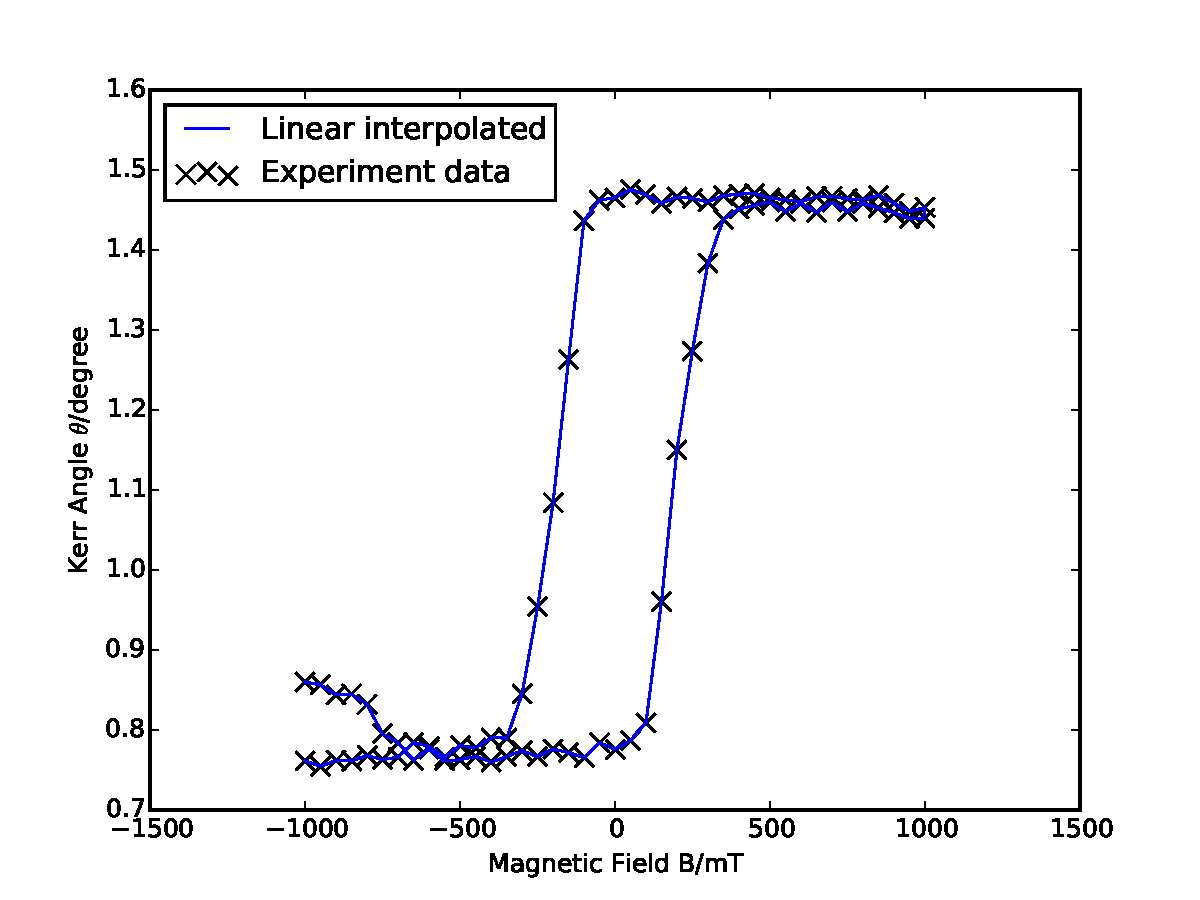
\includegraphics[width=\textwidth]{plot1.pdf}
    \caption{\label{fig:plot1}磁滞回线的线性插值图线,如图例所示,图中蓝线是为线性
        插值的磁滞回线图,十字状标定点是为实验测量数据.}
\end{figure}

\begin{figure}[htbp]
    \centering
    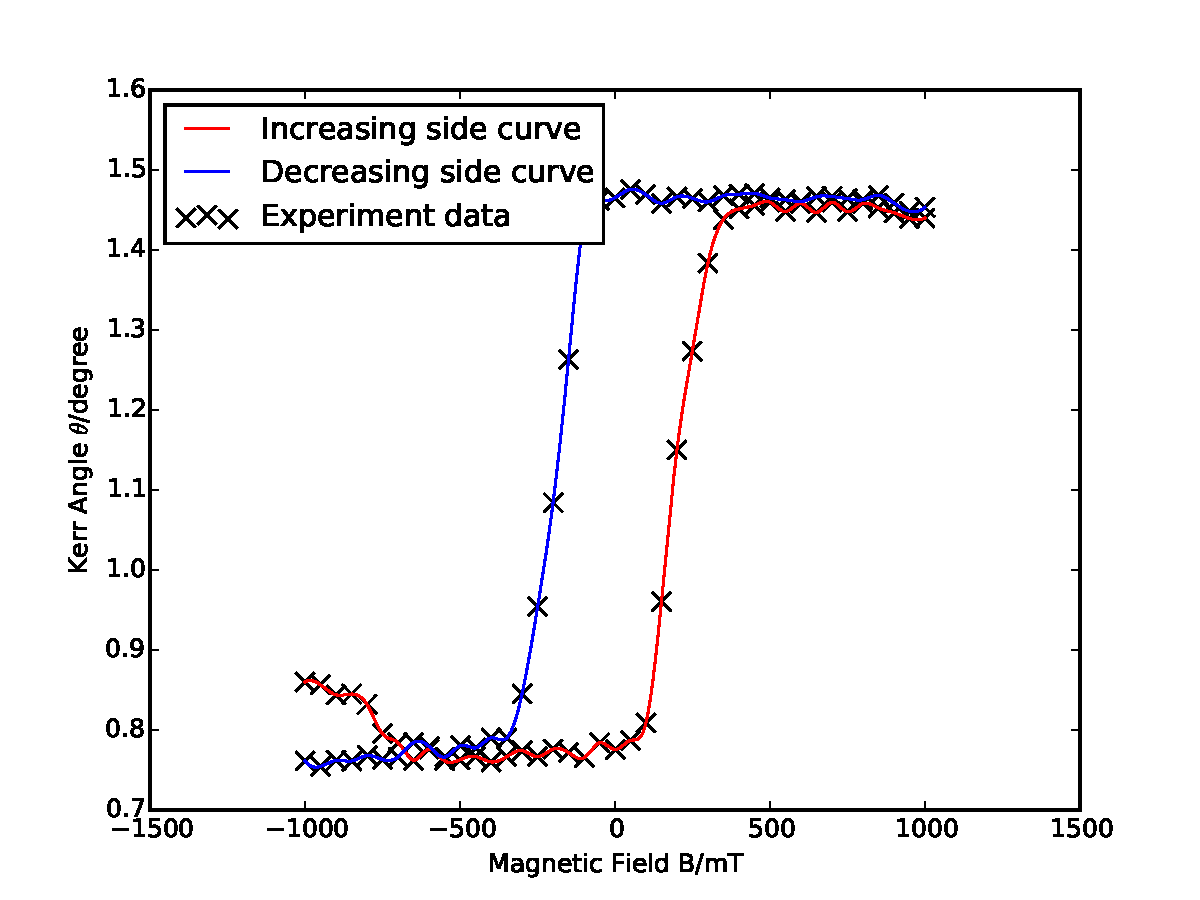
\includegraphics[width=\textwidth]{plot2.pdf}
    \caption{\label{fig:plot2}磁滞回线的样条插值图线,如图例所示,图中红线是为正向
        增大时的样条
        插值的磁滞回线图,蓝线是为负向
        减小时的样条
        插值的磁滞回线图,十字状标定点是为实验测量数据.}
\end{figure}

可以注意到,磁滞回线虽然在$B$轴方向上基本是以$B = 0$作为对称点的,但是在$\theta$轴
方向上并不是以零点为对称点,这是因为测量中存在转角的系统误差而导致的.这一系统误差
的主要来源应该是起偏器与检偏器的角度调节误差而引入的.

因此,数据处理中,首先取了所有数据点中最大和最小的5个点的角度值取平均,分别取为克尔
转角的最大值和最小值,然后二者取差除以二,从而消除这一系统偏差,将结果作为饱和克尔
转角的测量值.

测量得到饱和克尔转角为:
\begin{equation}
    \theta = \num{0.3555}^{\circ}
\end{equation}

另外,在数据处理中,分别对正向的样条差值曲线与负向的样条差值曲线求零点,得到了正向
和负向的矫顽力数值,正向矫顽力为
\begin{equation}
    H_+ = \num{1.507e5}{Am}
\end{equation}
负向矫顽力为
\begin{equation}
    H_- = \num{-1.511e5}{Am}
\end{equation}

二者绝对值的不同,应当是磁场测量由于霍尔探头的可能漂移和地磁场等因素而引入的误差
所导致的.

\section{结论}

本实验成功地测量了给定样品的克尔磁滞回线,并利用磁滞回线的测量数据计算了样品的饱
和克尔转角与矫顽力.


\section{致谢}
感谢周路群老师在实验中严谨而细致的指导.

感谢同组的刘照南同学认真而仔细的协助.

\begin{thebibliography}{}
\bibitem{Landau} L. D. Landau and E. M. Lifshitz and L. P. Pitaevskii,
Electrodynamics of Continuous Media, 2nd Edition, 世界图书出版公司(2007)
\bibitem{mo} R. Atkinson and P. H. Lissberger, Sign conventions in
magneto-optical calculations and measurements,Applied Optics, Vol.31 (1992)
6076.
\end{thebibliography}

\clearpage
\appendix
\section{思考题}

\begin{enumerate}
    \item 应该不一样高,因为锁相放大器对一次谐波分量和二次谐波分量的测量精度应该
        是不同的
    \item 输出的光强应当也具备周期性变化的特性,通过半波片的琼斯矩阵应当可以推算
        出来相关关系,理论上来说应该可以使用锁相放大器这一套系统进行复克尔转角的
        测量.
\end{enumerate}

\section{数据处理代码}

本实验的所有数据处理和绘图使用python语言完成.具体的处理使用了python的numpy,scipy
和matplotlib这数个开放源代码库套件.

相关的处理代码附在文后

\lstinputlisting[language=python]{data.py}

\end{document}
